% !TEX root = thesis.tex

\chapter{Basic dimension-independent operations}
\label{ch:operations-background}

\refch{ch:nd-modelling} identifies the most promising data structures in the context of a higher-dimensional GIS
and explains how certain fundamental operations are intimately related to the data structures for which they are defined.
This chapter therefore covers a number of basic dimension-independent operations, some of which need to be defined in the context of a specific data structure.
These operations are by themselves useful, as they correspond to common simple queries and modification.
In addition, some of them are used as building blocks for more complex operations described later in this thesis.

\refse{se:operations} introduces basic properties and operations on generalised/combinatorial maps and on Nef polyhedra, which are later respectively used for more complex higher-dimensional operations (\refchs{ch:extrusion},~\ref{ch:incremental-construction} \&~\ref{ch:linking-lods}) and for cleaning 2D and 3D data (\refch{ch:cleaning}).
\refse{se:ndmath} describes how to apply basic transformations to an $n$D simplicial/cell complex, which can be used to manipulate $n$D objects and to move around an $n$D scene (\refch{ch:slicing}).

\refse{se:spatial-indexing} describes some spatial indexing methods which can be applied to higher-dimensional objects, allowing a system to solve two common problems: keeping track of disconnected objects and efficiently obtaining the objects in a particular region.
\refse{se:duality} discusses how the concept of duality works in higher dimensions, which can be used to characterise the relationships between objects of any dimension.
\refse{se:ndqueries} puts the concepts of this chapter into practice by providing a few concrete examples of simple dimension-independent operations, including a technique to quickly compare objects in any dimension, which is itself used as the basis of the incremental construction operation in \refch{ch:incremental-construction}.
These examples showcase how operations on an ordered topological model are remarkably efficient compared to the same operations on a Simple Features-like representation.

Most of \refse{se:duality} is based on the paper:
\begin{itemize}
\papergeoadvancesnd%
\end{itemize}

\section{Basic operations on certain data structures}
\label{se:operations}

\subsection{Generalised and combinatorial maps}
\label{ss:operations-maps}

As described in \refse{ss:ordered-topological-models}, an object in an ordered topological model is described as a set of combinatorial simplices, which are connected by a set of predefined relations.
These relations and the operations that use them are described in more detail below, partly based on the definitions used in \citet{Damiand14}.
Note however that some of the definitions presented here are somewhat simplified, as they are meant only to handle the types of representations and further operations used in this thesis.

In the case of a generalised map, which is shown in \reffig{fig:2dcc}, all the relations between darts take the form of \emph{involutions}---bijective functions that are their own inverse.
That is, they are functions $f$ such that $f\big(f(x)\big) = x$, or equivalently $f = f^{-1}$.
\begin{figure}[tbp]
\centering
\subfloat[]{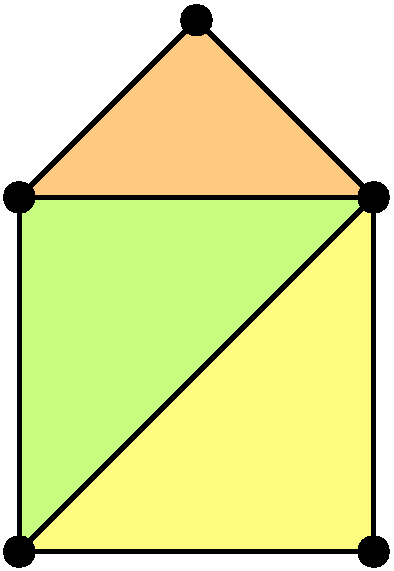
\includegraphics[width=0.3\linewidth]{figs/2dcc}}
\quad
\subfloat[]{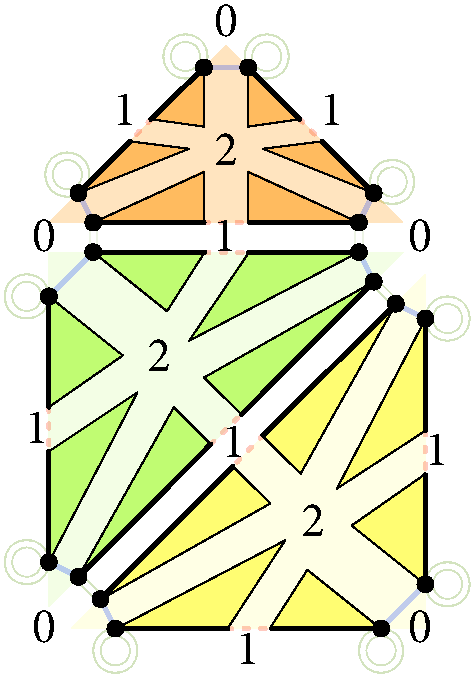
\includegraphics[width=0.3\linewidth]{figs/2dcc-gmap}}
\quad
\subfloat[]{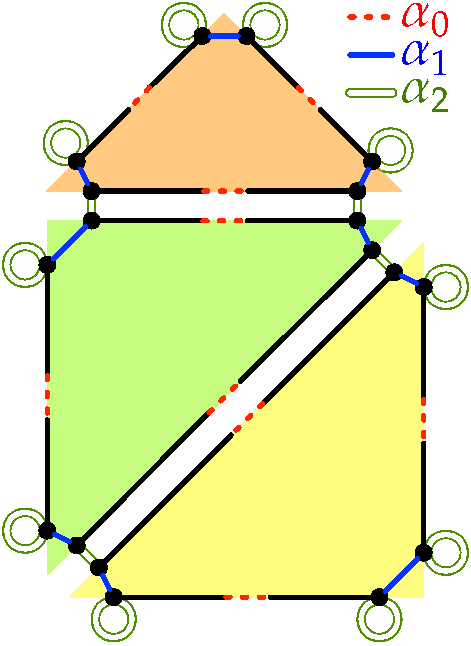
\includegraphics[width=0.3\linewidth]{figs/2dcc-alphas}}
\caption[Involutions in a 2D generalised map]{For (a) 2D cell complex represented as a 2D generalised map (b) in a simplicial complex-based depiction as used in \refse{ss:ordered-topological-models}, (c) in a simpler depiction using half-edges and showing explicitly the relations between the darts.
As involutions are pairwise relations between darts, they are their own inverse, \ie\ applying them twice means returning to the original dart.}
\label{fig:2dcc}
\end{figure}
In addition, certain darts are $i$-free, which means that for a given dart $d$, $\alpha_i(d) = d$.
These darts represent the boundary of the map.

More formally, a $n$-dimensional generalised map is defined as a $(n+2)$-tuple $G = (D,\alpha_{0},\ldots,\alpha_{n})$, where:

\begin{itemize}
\item
$D$ is a finite set of darts;

\item
$\forall 0 \leq i \leq n$, $\alpha_{i}$ is an involution on $D$;

\item
$\forall 0 \leq i \leq n-2, \forall i+2 \leq j \leq n$, $\alpha_{i}\circ \alpha_{j}$ is an involution on $D$.
\end{itemize}

In a combinatorial map, the relations between the darts are somewhat different.
As shown in \reffig{fig:cmap-free}, polygonal curves in a combinatorial map result in some darts that have an undefined $\beta_1$ relation.
\marginpar{
\captionsetup{type=figure}
\centering
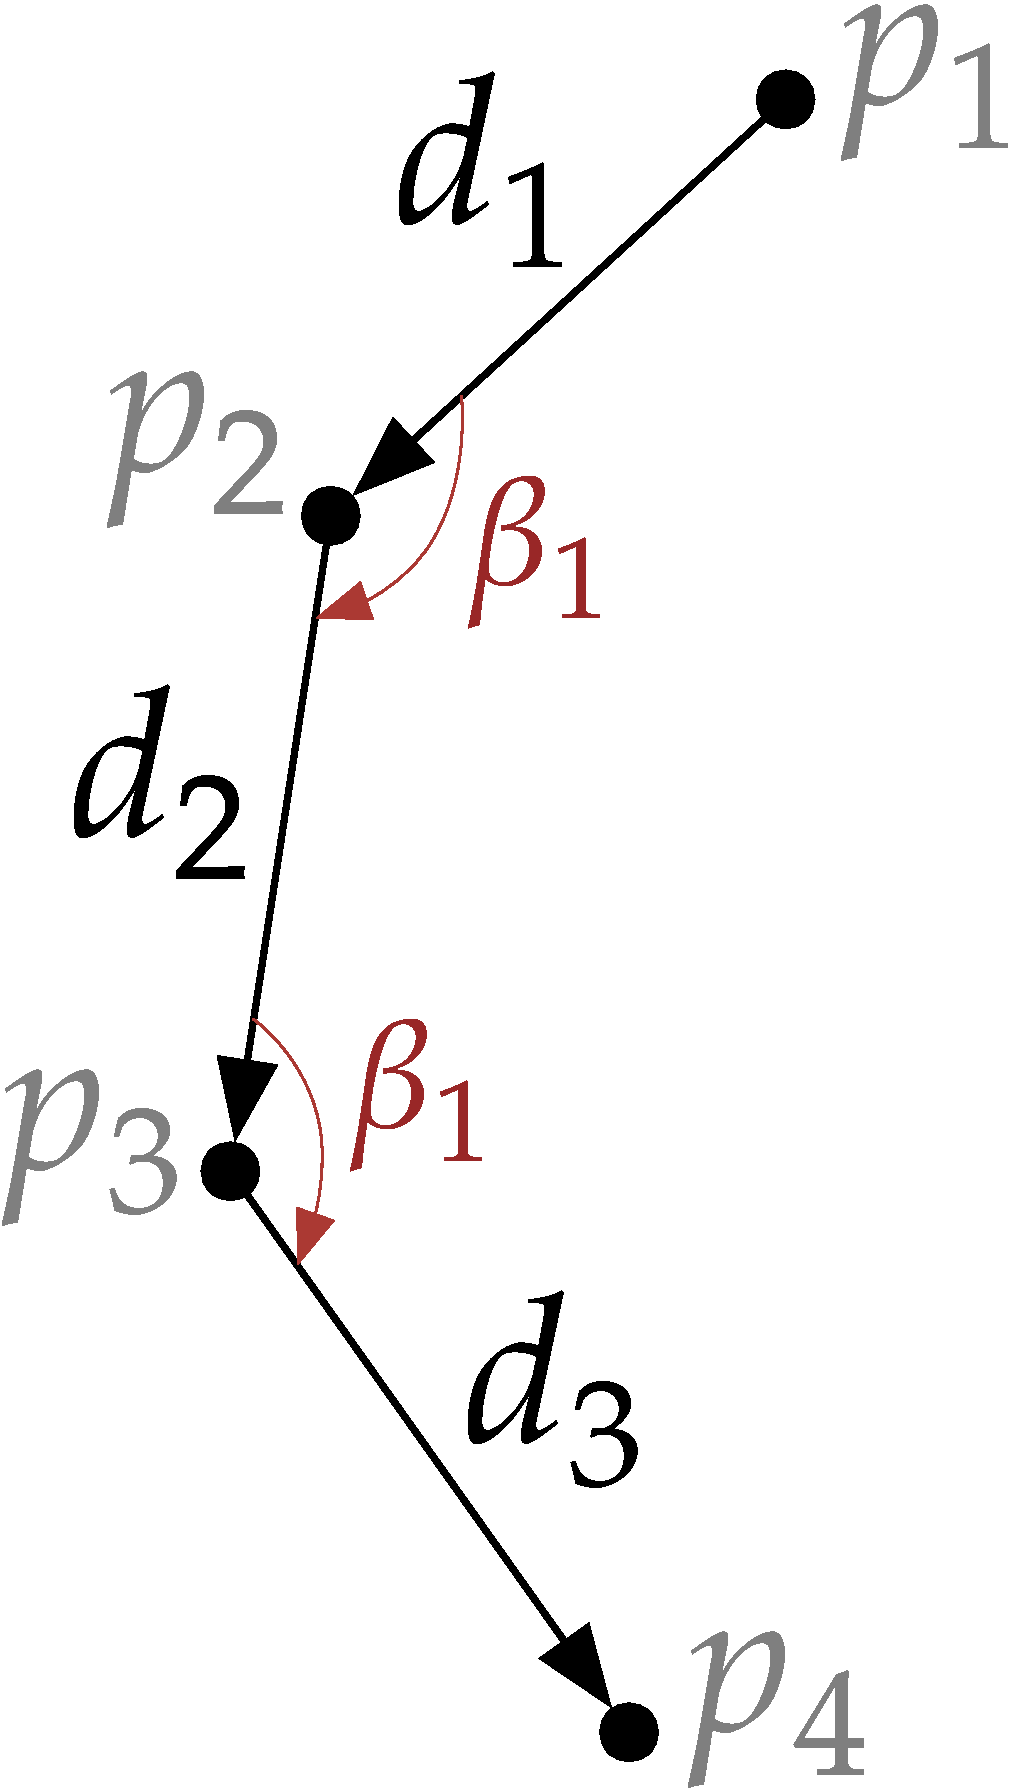
\includegraphics[width=\marginparwidth]{figs/cmap-free}
\caption[Partial permutations in a 1D combinatorial map]{The $\beta_1$ relations in a 1D combinatorial map are partial permutations. Whereas $\beta_1(d_1) = d_2$ and $\beta_1(d_2) = d_3$, $\beta_1(d_3) = \emptyset$.}
\label{fig:cmap-free}
}
For a given dart $d$ with an undefined relation $\beta_1$, this is encoded as $\beta_1(d) = \emptyset$ and the dart is said to be $1$-free.
Because of this, the $\beta_1$ relations in a combinatorial map do not form involutions, but instead form only \emph{partial permutations}.
% When ... he darts joined by $\beta_1$ relations consist of a subset of the darts in the map which form a \emph{cyclic permutation}, \ie\ they are connected to each other so as to form one cycle, which effectively represents the edges around a face.
In addition, as shown in \reffig{fig:2dcc-betas}, in a combinatorial map of any dimension, the darts that lie on the boundary of the map also have certain undefined $\beta$ relations, which are linked to the special value $\emptyset$.
\marginpar{
\captionsetup{type=figure}
\centering
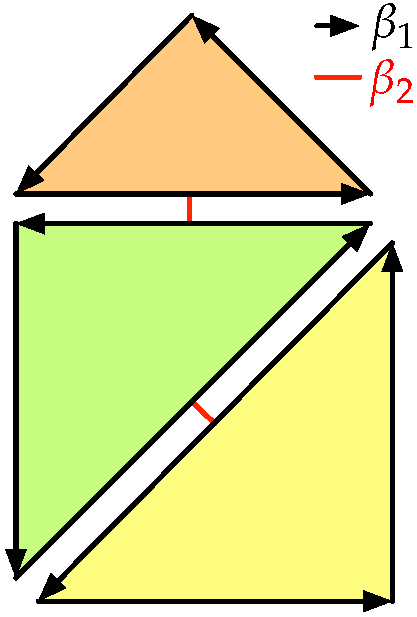
\includegraphics[width=\marginparwidth]{figs/2dcc-betas}
\caption[Partial permutations in a 2D combinatorial map]{The $\beta_1$ relations in a 2D combinatorial map are partial permutations, the $\beta_2$ relations are partial involutions.}
\label{fig:2dcc-betas}
}
If a given $\beta_i(d) = \emptyset$, the dart $d$ is said to be $i$-free.
Because of the existence of these relations, the $\beta$ relations of a combinatorial map other than $\beta_1$ form \emph{partial involutions}.

More formally, an $n$-dimensional combinatorial map is defined as an $(n+1)$-tuple $C = (D, \beta_{1}, \ldots, \beta_{n})$ where:

\begin{itemize}
\item
$D$ is a finite set of darts;

\item
$\beta_{1}$ is a partial permutation on $D$;

\item
$\forall 2 \leq i \leq n$, $\beta_{i}$ is a partial involution on $D$;

\item
$\forall 0 \leq i \leq n-2, \forall 3 \leq j \leq n$, $i+2 \leq j$, $\beta_{i}\circ \beta_{j}$ is a partial involution on $D$.
\end{itemize}

The properties of generalised and combinatorial maps are crucial, as when they are enforced, they ensure that darts form a valid combinatorial structure.
They also allow the definition of various operations that operate on the combinatorial structures induced by the darts and their relations.
Many of these operations are based on the concept of an \emph{orbit}, a subset of the darts of a generalised/combinatorial map that are connected by certain relations.
Starting from a given dart $d$ and a set of relations $\Alpha$, the orbit $\langle\Alpha\rangle(d)$ obtains all the darts that can be reached by recursively following all relations in $\Alpha$.
% operations are described below.

\begin{description}

\item[Darts of a cell]
Considering that cells in a generalised or combinatorial map are represented by \emph{sets of darts}, an important basic operation is obtaining all the darts that represent a given cell of any dimension.
In a generalised map, from a given dart $d$ known to be part of an $i$-cell, the darts of the $i$-cells are those that can be reached by recursively following all relations \emph{except} for $\alpha_i$.
As shown in \reffig{fig:darts-of-cell}, this is given by the orbit $\langle\alpha_0, \ldots, \alpha_{i-1}, \alpha_{i+1}, \ldots, \alpha_n\rangle(d)$.
In a combinatorial map, due to the oriented nature of the $\beta_1$ relations, in order to obtain the darts of a $0$-cell it is instead necessary to follow a composition of relations given by $\langle \{\beta_j\circ \beta_k \mid \forall 1 \leq k \leq n, \forall 1 \leq j \leq k\} \rangle(d)$.
The cells of dimension two and higher are obtained in a similar manner as in a generalised map, by following all relations \emph{except} for $\beta_i$, \ie\ $\langle\beta_1, \ldots, \beta_{i-1}, \beta_{i+1}, \ldots, \beta_n\rangle(d)$.
\begin{figure}[tbp]
\centering
\subfloat[]{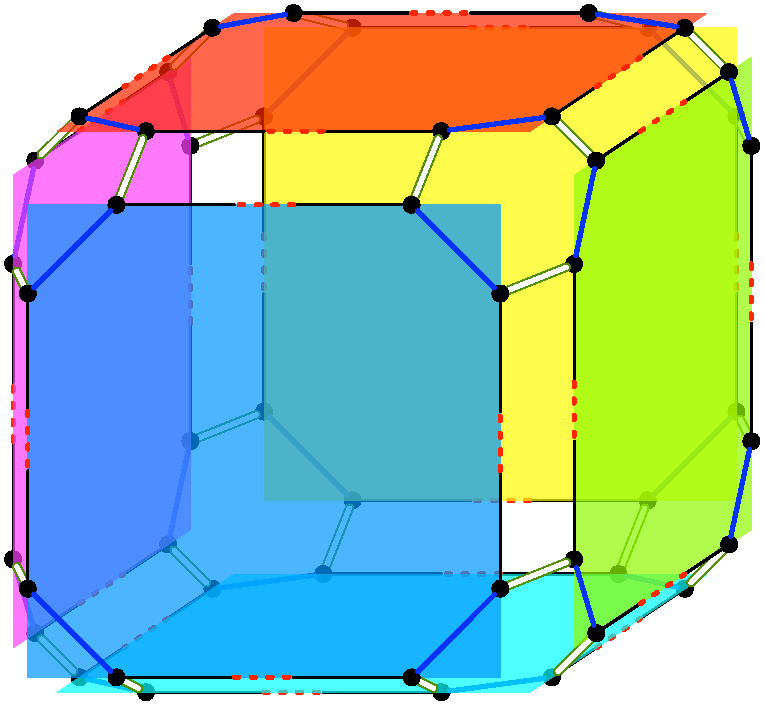
\includegraphics[width=0.45\linewidth]{figs/darts-of-cell-1}}
\quad
\subfloat[]{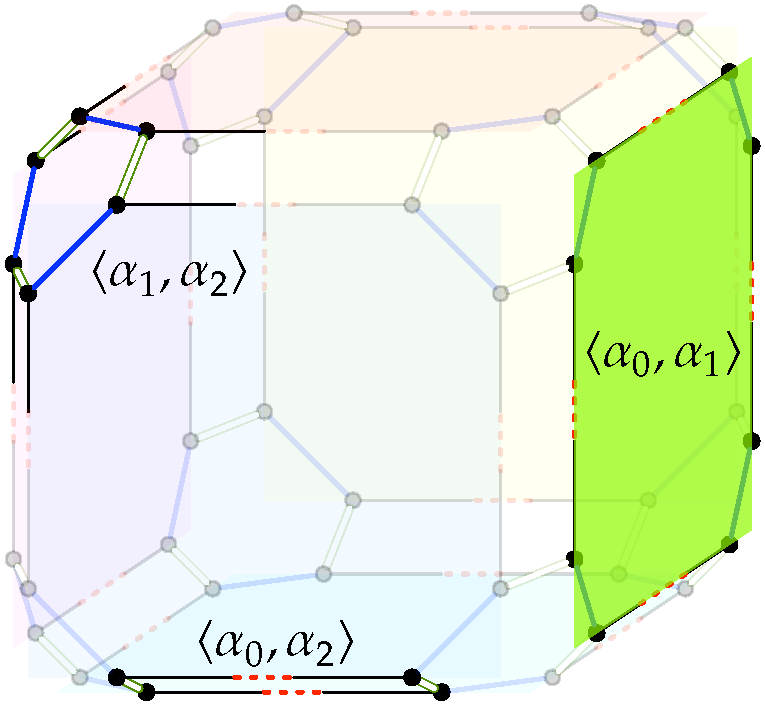
\includegraphics[width=0.45\linewidth]{figs/darts-of-cell-2}}
\caption[Darts of a cell]{Starting from (a) a 2D generalised map representation of a cube, all the darts representing an $i$-cell of the map can be obtained by starting from any dart known to be part of the $i$-cell, then using the orbit that contains all relations but $\alpha_i$. (b) Here, the orbits of a specific 0-cell, 1-cell and 2-cell.}
\label{fig:darts-of-cell}
\end{figure}

\item[Isomorphism]
It is possible to check if two maps are \emph{isomorphic} by finding whether there is a one-to-one mapping between the darts in the maps that also preserves the relations between them.
That is, given two generalised maps $(D,\alpha_{0},\ldots,\alpha_{n})$ and $(D^\prime,\alpha_{0}^\prime,\ldots,\alpha_{n}^\prime)$, an isomorphism is a function $f: D \rightarrow D^\prime$ such that $\forall d \in D, \forall 0 \leq i \leq n, f\big(\alpha_i\left(d\right)\big) = \alpha_i^\prime\left(f\left(d\right)\right)$.
Similarly, given two combinatorial maps $(D, \beta_{1}, \ldots, \beta_{n})$ and $(D^\prime, \beta_{1}^\prime, \ldots, \beta_{n}^\prime)$, an isomorphism is a function $f: D \cup \left\{\emptyset\right\} \rightarrow D^\prime \cup \left\{\emptyset\right\}$ such that $f(\emptyset) = \emptyset$, and else $\forall d \in D, \forall 1 \leq i \leq n, f\left(\beta_i\left(d\right)\right) = \beta_i^\prime\left(f\left(d\right)\right)$.

\item[Sewable darts]
Starting from isolated darts, these can be assembled together via the sewing operation, described below.
However, it is important to first determine if they can be sewed together along a given dimension.
Given a generalised map $(D,\alpha_{0},\ldots,\alpha_{n})$ and two darts from the map $d,d^\prime \in D$, $d$ and $d^\prime$ are $i$-sewable if and only if $d \neq d^\prime$, $d$ and $d^\prime$ are $i$-free, and there is an isomorphism between $\langle\alpha_0, \ldots, \alpha_{i-2}, \alpha_{i+2}, \ldots, \alpha_n\rangle(d)$ and $\langle\alpha_0, \ldots, \alpha_{i-2}, \alpha_{i+2}, \ldots, \alpha_n\rangle(d^\prime)$ such that $f(d) = d^\prime$.
Similarly, given a combinatorial map $(D, \beta_{1}, \ldots, \beta_{n})$ and two darts from the map $d,d^\prime \in D$, $d$ and $d^\prime$ are $i$-sewable if and only if $d \neq d^\prime$, $d$ and the inverse of $d^\prime$ are $i$-free, and there is an isomorphism between $\langle\beta_1, \ldots, \beta_{i-2}, \beta_{i+2}, \ldots, \beta_n\rangle(d)$ and $\langle\beta_1, \ldots, \beta_{i-2}, \beta_{i+2}, \ldots, \beta_n\rangle(d^\prime)$ such that $f(d) = d^\prime$.

\item[Sewing]
The sewing operation is the basic construction method used to link isolated darts in a map in order to form cell complexes.
Intuitively, it is possible to link two $i$-cells along a common $(i-1)$-cell by sewing corresponding darts on the common $(i-1)$-cell on each $i$-cell.
\begin{figure}[tbp]
\centering
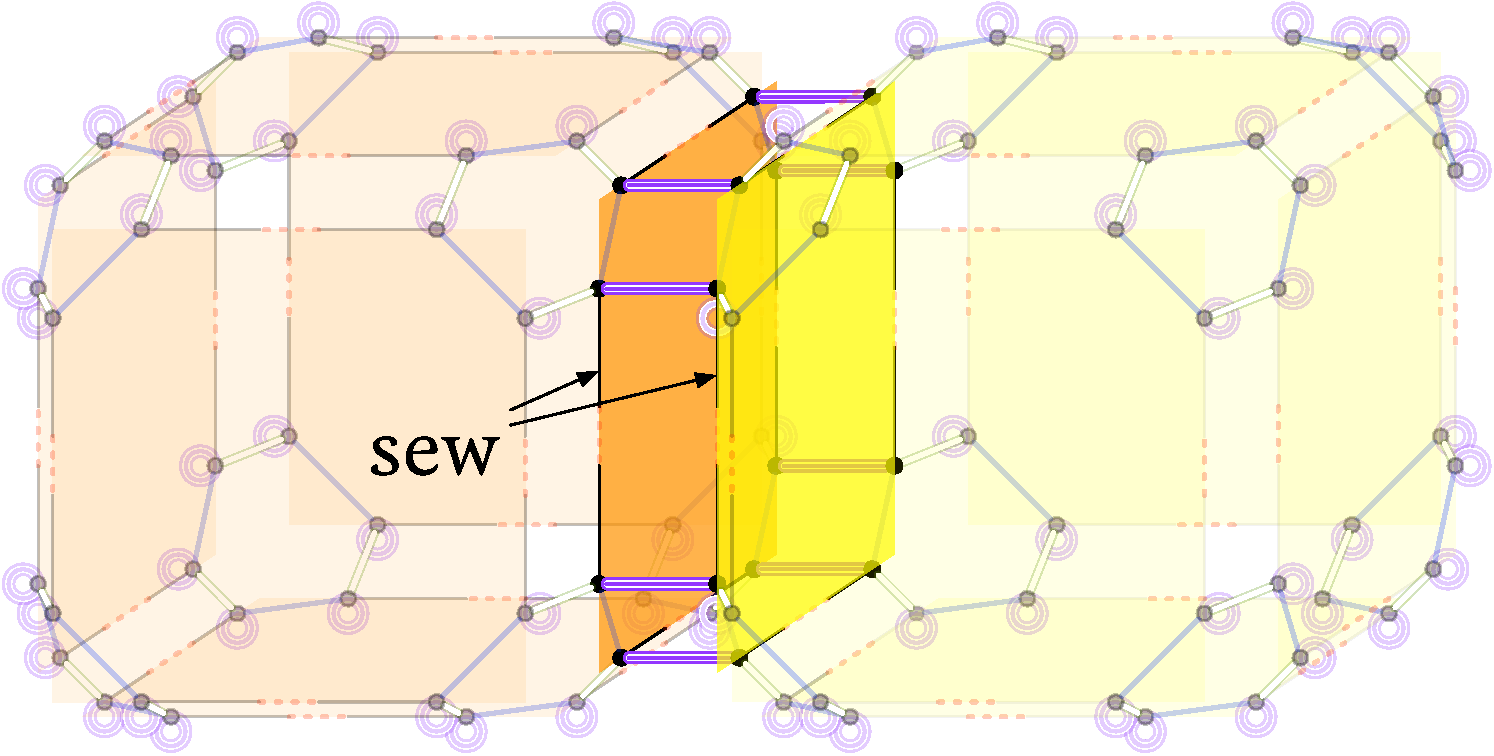
\includegraphics[width=\linewidth]{figs/3-sew}
\caption[3-sewing two cubes]{Two cubes in a 3D generalised map can be linked together by 3-sewing corresponding darts on the common face (highlighted) on each cube. This operation uses the orbits of each face on each cube in order to link the corresponding darts.}
\end{figure}
Given a generalised map $(D,\alpha_{0},\ldots,\alpha_{n})$ and two darts $d,d^\prime \in D$ that are $i$-sewable using the isomorphism $f$, $i$-sewing $d$ and $d^\prime$ means that $\forall e \in \langle\alpha_0, \ldots, \alpha_n\rangle(d)$, $\alpha_i(e)$ should be set to $f(e)$ and $\alpha_i\big(f(e)\big)$ should be set to $e$.
Given a combinatorial map $(D, \beta_{1}, \ldots, \beta_{n})$ and two darts $d,d^\prime \in D$ that are $1$-sewable using the isomorphism $f$, $1$-sewing $d$ and $d^\prime$ means that $\forall e \in \langle \{\beta_i\circ \beta_j \mid \forall 3 \leq k \leq n, \forall 3 \leq j \leq k\} \rangle(d)$, $\beta_1(e)$ should be set to $f(e)$ and $\forall e^\prime \in \langle \{\beta_i\circ \beta_j \mid \forall 3 \leq k \leq n, \forall 3 \leq j \leq k\} \rangle(d^\prime)$, $\beta_1(f(e^\prime))$ should be set to $e^\prime$.
For the cells of dimension two and higher, if $d$ and $d^\prime$ are $i$-sewable ($i \geq 2$), $i$-sewing them means that $\forall e \in \langle\beta_{1}, \ldots, \beta_{n}\rangle(d)$, $\beta_i(e)$ should be set to $f(e)$ and $\beta_i\big(f(e)\big)$ should be set to $e$.

\end{description}

\subsection{Nef polyhedra}
\label{ss:operations-nef}

As discussed in \refse{ss:implicit-models}, Nef polyhedra \citep{Nef78,Bieri88} are able to represent polytopes of any dimension based on a set of local pyramids, which contain the neighbourhood information around each vertex.
Despite the fact that---to the best of my knowledge---there is no available implementation of Nef polyhedra in more than three dimensions, their dimension-independent formulation and the relative ease of implementing \emph{robust} operations on Nef polyhedra nevertheless make them valuable in a higher-dimensional setting.

In particular, Boolean set operations on 2D Nef polygons and 3D Nef polyhedra are very useful to obtain valid 2D and 3D datasets---something that will be shown in \refse{se:3drepair}.
These \emph{clean} datasets can then be used as a base for higher-dimensional ones, either by extruding them (\refch{ch:extrusion}), by using them to define parts of a higher-dimensional object's boundary (\refch{ch:incremental-construction}), or by linking corresponding datasets that represent other points in scale or time (\refch{ch:linking-lods}), among other possibilities.

The key advantage of operations on Nef polyhedra is the fact that many of them can be largely implemented at the local pyramid level.
As shown by \citet{Seel01} in 2D and \citet{Hachenberger06} in 3D, Boolean set operations are one such case.
Based on the approach advocated by \citet{Rossignac89}, it is possible to compute these type of binary (or $n$-ary) operations in three steps: subdivision, selection and simplification.
The \emph{subdivision} is the most complex of these.
It consists of computing an overlay of the input polyhedra, creating the overall structure where the result will be put (\eg\ the vertices, edges, faces and volumes of a cell complex).
This can be computed with the methods used for arrangements of line segments in 2D \citep[\S{}8.3]{deBerg08}, or by computing line-segment-to-line-segment and line-segment-to-polygon intersections in 3D \citep{Hachenberger06}, which give the locations of the new vertices and thus the new local pyramids.

After this, the \emph{selection} step computes whether the individual cells are to be considered as part of the output or not (\ie\ whether they are in the interior or exterior of the Nef polygons/polyhedra).
The \emph{simplification} removes unnecessary structures in way that does not alter the point set that is represented, akin to the dissolving operations common in GIS.\@
% In the case of \citet{Hachenberger06}, it also involves solving conflicts and computing the missing information

\reffig{fig:nef-boolean} shows an example how this works in practice in 2D.
Starting from two Nef polygons $A$ and $B$, each of which is stored as the local pyramids of its vertices, the intersections between their line segments are computed.
As shown previously in \reffigp{fig:nef}, each of these 2D local pyramids can be stored as a list of 1D intervals\footnote{Which reduces the dimensionality of the problem by one.}.
Using the vertices of each polygon, as well as these intersections, additional local pyramids for each polygon are obtained.
A Boolean set operation is then computed by computing it on the local pyramids of the input.
Finally, unnecessary local pyramids can be removed from the output (\eg\ local pyramid $f$ in $A \cup B$, which represents a half-space and thus does not lie on an output vertex).
\begin{figure}[tb]
\centering
\subfloat[]{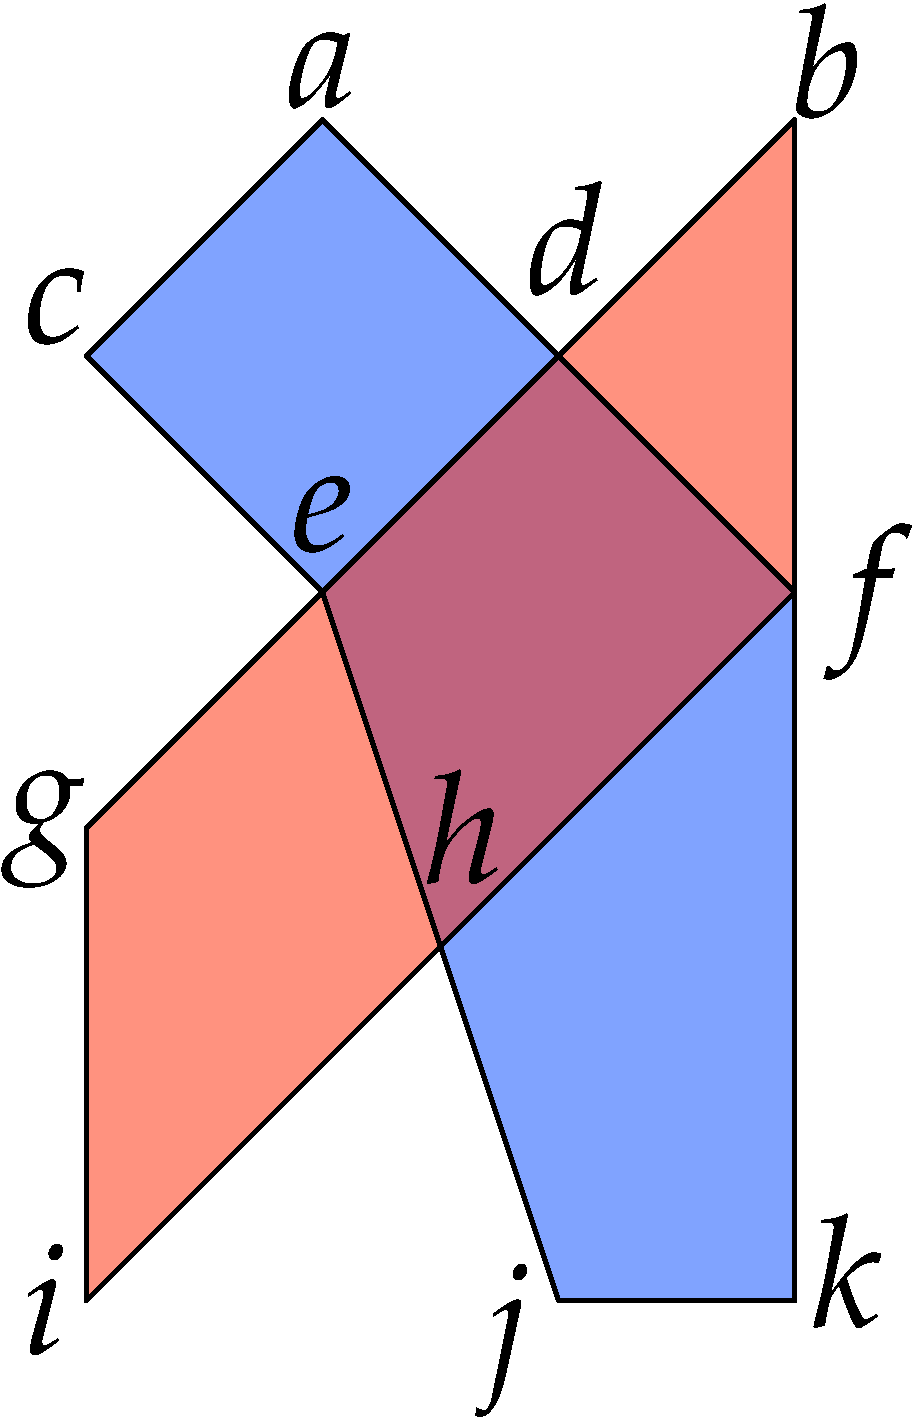
\includegraphics[scale=0.19]{figs/nef-boolean-1}}
\quad
\subfloat[]{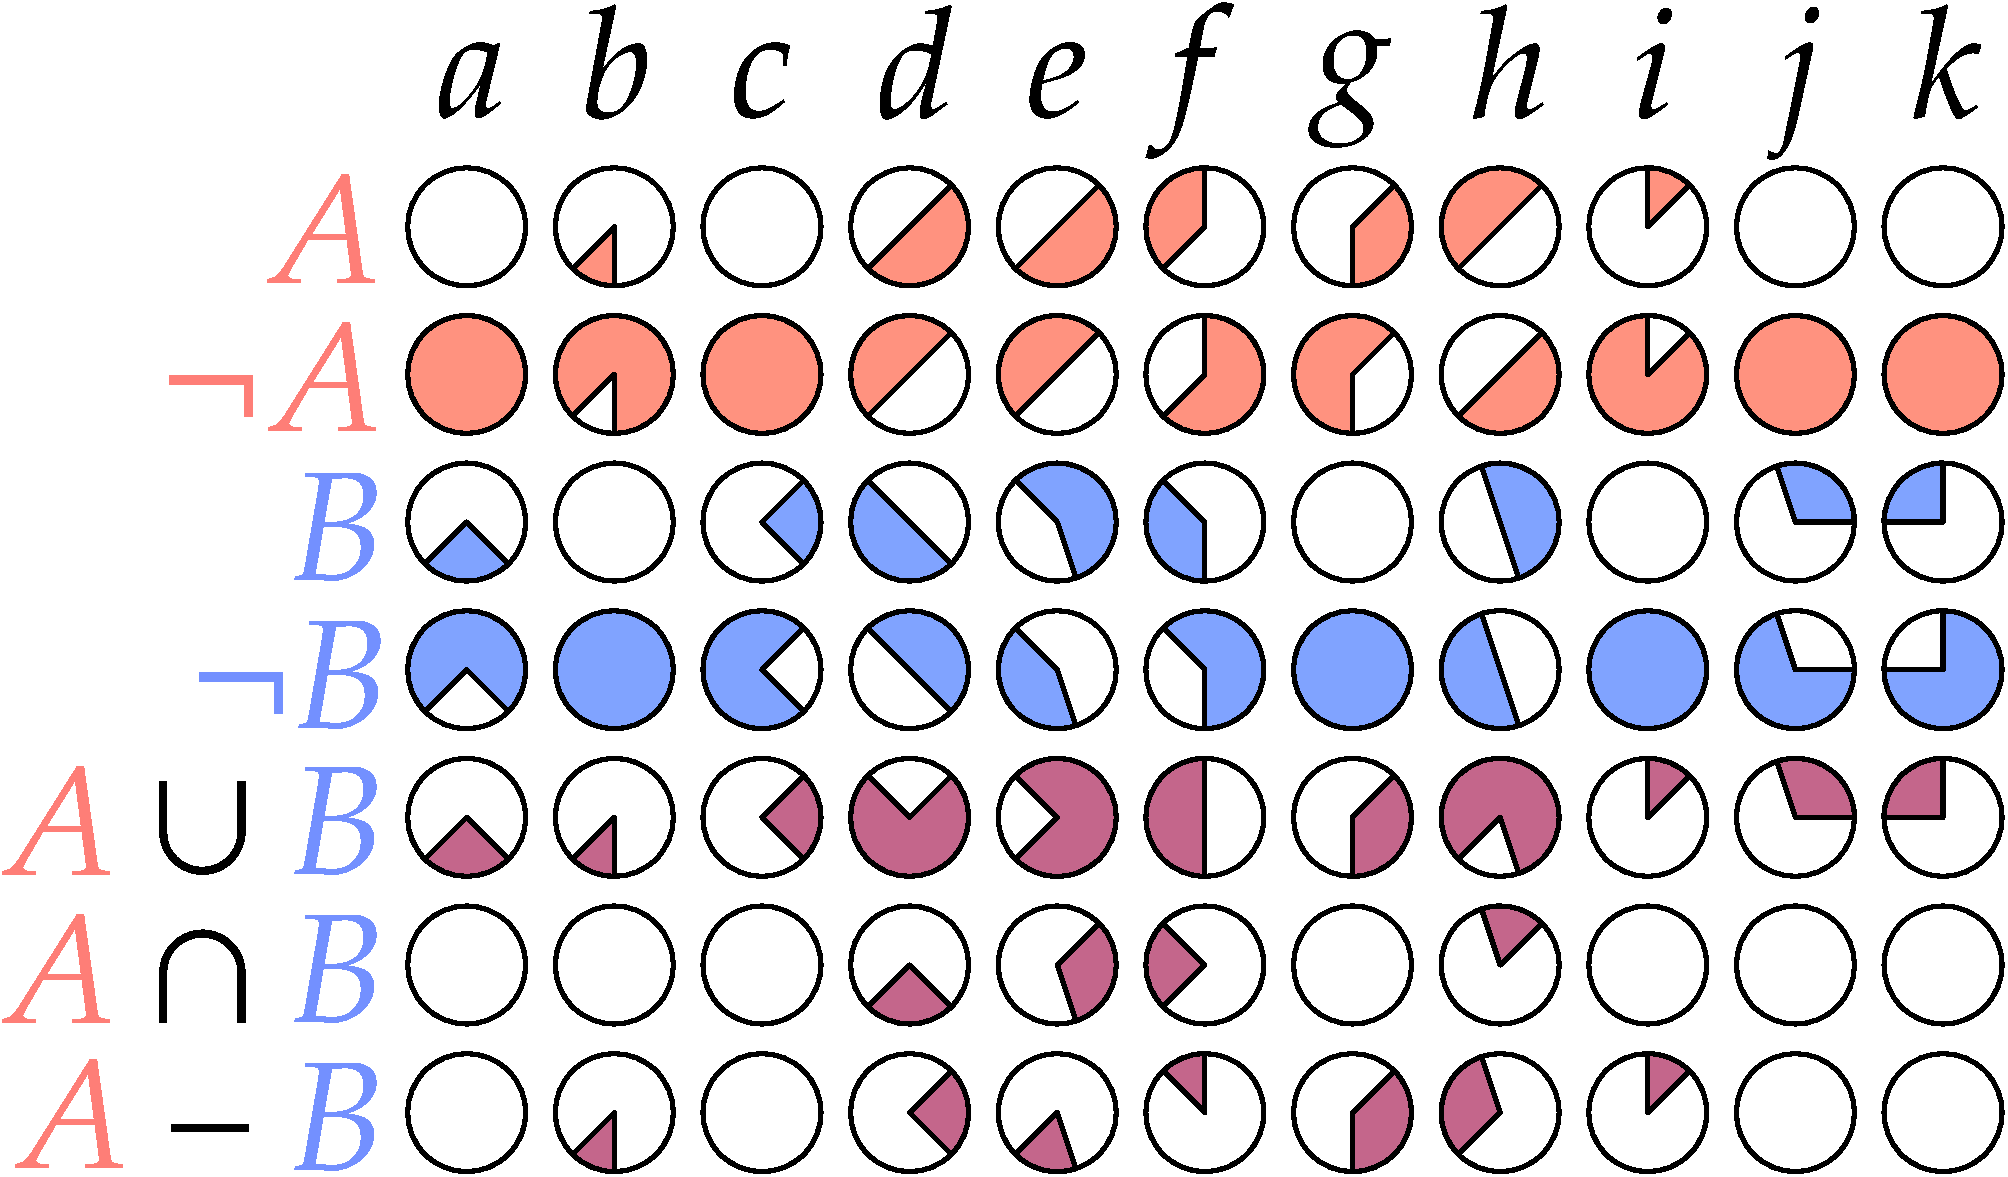
\includegraphics[scale=0.19]{figs/nef-boolean-2}}
\caption[Boolean set operations on Nef polygons]{Various Boolean set operations on (a) the Nef polygons $A$ (red) and $B$ (blue) that can be performed on (b) their local pyramids: complement ($\neg$), union ($\cup$), intersection ($\cap$) and difference ($-$).}
\label{fig:nef-boolean}
\end{figure}

\section{Basic transformations of an $n$D scene}
\label{se:ndmath}

Starting from an $n$-dimensional simplicial complex or cell complex with linear geometry, where every vertex is embedded in a location in $\mathbb{R}^n$, it is possible to define a set of basic transformations to manipulate $n$D objects simply by applying them to the coordinates of every vertex.
This section thus describes dimension-independent versions of the three most important transformations to an $\mathbb{R}^n$ point set: \emph{translation}, \emph{rotation} and \emph{scaling}.
In addition, it explains how compute the \emph{cross-product} in higher dimensions, which is later used to compute a vector that is orthogonal to all of a set of other vectors.

\textbf{Translating} of a set of points in $\mathbb{R}^n$ can be easy expressed as a sum with a vector $t = \left[t_0, \ldots, t_n\right]$, or alternatively as a multiplication with a matrix using homogeneous coordinates, which is defined as:

\begin{equation*}
T = \begin{bmatrix}
1 & 0 & \cdots & 0 & t_0 \\
0 & 1 & \cdots & 0 & t_1 \\
\vdots & \vdots & \ddots & \vdots & \vdots \\
0 & 0 & \cdots & 1 & t_n \\
0 & 0 & \cdots & 0 & 1 \\
\end{bmatrix}
\end{equation*}

In particular, it is often useful to apply a multiplication with a \emph{centering matrix} \citep[\S{}3.2]{Marden96}, which  moves a dataset to a position around the origin.
Such a matrix would be defined as $\mathbb{I}_n - \frac{1}{n}\mathbb{1}$, where $\mathbb{I}$ is the identity matrix and $\mathbb{1}$ is a matrix where all entries are set to 1.

\textbf{Scaling} is similarly simple.
Given a vector $s = \left[ s_0, s_1, \ldots, s_n \right]$ that defines a scale factor per axis (which in the simplest case can be the same for all axes), it is possible to define a matrix to scale an object as:

\begin{equation*}
S = \begin{bmatrix}
s_0 & 0 & \cdots & 0 \\
0 & s_1 & \cdots & 0 \\
\vdots & \vdots & \ddots & \vdots \\
0 & 0 & \cdots & s_n \\
\end{bmatrix}
\end{equation*}

\textbf{Rotation} is somewhat more complex.
Rotations in 3D are often conceptualised intuitively as rotations \emph{around an axis}.
As there are three degrees of rotational freedom in 3D, combining three such elemental rotations can be used to describe any rotation in 3D space.
Most conveniently, these three rotations can be performed respectively around the $x$, $y$ and $z$ axes, such that a point's coordinate on the axis being rotated remains unchanged.
This is a very elegant formulation, but this view of the matter is only valid in 3D.

A more correct way to conceptualise rotations is to consider them as rotations \emph{parallel to a given plane} \citep{Hollasch91}, such that a point that is continuously rotated (without changing rotation direction) will form a circle that is parallel to that plane.
This view is valid in 2D (where there is only one plane), in 3D (where the plane is orthogonal to the axis of rotation) and in any higher dimension.
Incidentally, this shows that the degree of rotational freedom in $n$D is given by the number of possible combinations of two axes (which define a plane) on that dimension \citep{Hanson94}, \ie\ $\binom{n}{2}$.
A general rotation in any dimension can also be seen as a sequence of elementary rotations, although the total number of these rotations that need to be performed increases significantly.

Considering the 2D rotation matrix $R_{xy}$ that rotates points in $\mathbb{R}^2$ parallel to the $xy$ plane:

\begin{equation*}
R_{xy} = \begin{bmatrix}
\cos \theta & -\sin \theta \\
\sin \theta & \cos \theta \\
\end{bmatrix}
\end{equation*}

It is possible to obtain the three 3D rotation matrices to rotate points in $\mathbb{R}^3$ around the $x$, $y$ and $z$ axes, which correspond to the rotations parallel to the $yz$, $zx$ and $xy$ planes\footnote{Note the order of $zx$, which follows the right hand rule and defines the signs of the sines in the rotation matrices.}.
These would consist of an identity row and column that preserves the coordinate of a particular axis and rotates the coordinates of the other two, resulting in the following three 3D rotation matrices:

\hspace{-\marginparwidth}\hspace{-\marginparsep}\makebox[\overflowingheadlen][l]{
\begin{minipage}{\overflowingheadlen}
\begin{align*}
R_{yz} &= \begin{bmatrix}
1 & 0 & 0 \\
0 & \cos \theta & -\sin \theta \\
0 & \sin \theta & \cos \theta \\
\end{bmatrix} &
R_{zx} &= \begin{bmatrix}
\cos \theta & 0 & \sin \theta \\
0 & 1 & 0 \\
-\sin \theta & 0 & \cos \theta \\
\end{bmatrix} & 
R_{xy} &= \begin{bmatrix}
\cos \theta & -\sin \theta & 0 \\
\sin \theta & \cos \theta & 0 \\
0 & 0 & 1 \\
\end{bmatrix}
\end{align*}
\end{minipage}
}

Similarly, in a 4D coordinate system defined by the axes $x$, $y$, $z$ and $w$, it is possible to define six 4D rotation matrices, which correspond to the six rotational degrees of freedom in 4D \citep{Hanson94}.
These respectively rotate points in $\mathbb{R}^4$ parallel to the $xy$, $xz$, $xw$, $yz$, $yw$ and $zw$ planes:

\hspace{-\marginparwidth}\hspace{-\marginparsep}\makebox[\overflowingheadlen][l]{
\begin{minipage}{\overflowingheadlen}
\begin{align*}
R_{xy} &= \begin{bmatrix}
\cos \theta & -\sin \theta & 0 & 0 \\
\sin \theta & \cos \theta & 0 & 0 \\
0 & 0 & 1 & 0 \\
0 & 0 & 0 & 1 \\
\end{bmatrix} & 
R_{xz} &= \begin{bmatrix}
\cos \theta & 0 & -\sin \theta & 0 \\
0 & 1 & 0 & 0 \\
\sin \theta & 0 & \cos \theta & 0 \\
0 & 0 & 0 & 1 \\
\end{bmatrix} & 
R_{xw} &= \begin{bmatrix}
\cos \theta & 0 & 0 & -\sin \theta \\
0 & 1 & 0 & 0 \\
0 & 0 & 1 & 0 \\
\sin \theta & 0 & 0 & \cos \theta \\
\end{bmatrix} \\
% \end{align*}
% \end{minipage}
% \begin{minipage}{\overflowingheadlen}
% \begin{align*}
R_{yz} &= \begin{bmatrix}
1 & 0 & 0 & 0 \\
0 & \cos \theta & -\sin \theta & 0 \\
0 & \sin \theta & \cos \theta & 0 \\
0 & 0 & 0 & 1 \\
\end{bmatrix} & 
R_{yw} &= \begin{bmatrix}
1 & 0 & 0 & 0 \\
0 & \cos \theta & 0 & -\sin \theta \\
0 & 0 & 1 & 0 \\
0 & \sin \theta & 0 & \cos \theta \\
\end{bmatrix} & 
R_{zw} &= \begin{bmatrix}
1 & 0 & 0 & 0 \\
0 & 1 & 0 & 0 \\
0 & 0 & \cos \theta & -\sin \theta \\
0 & 0 & \sin \theta & \cos \theta \\
\end{bmatrix} \\
\end{align*}
\end{minipage}
}

This scheme of a set of elementary rotations can be easily extended to any dimension, always considering a rotation matrix as a transformation that rotates two coordinates of every point and maintains the coordinates of all other coordinates.
An alternative could be to apply more than one rotation at a time, which is possible in higher dimensions \citep{vanElfrinkhof97}.
However, for an application expecting user interaction, it might be more intuitive to rely on a rotation plane that does not correspond to specific axes, \eg\ by defining such a plane through a triplet of points \citep{Hanson94}.

The \textbf{cross-product} is easier to understand by first considering the lower-dimensional cases.
In 2D, it is possible to obtain a normal vector to a 1D line as defined by two (different) points $p^0$ and $p^1$, or equivalently a normal vector to a vector from $p^0$ to $p^1$.
In 3D, it is possible to obtain a normal vector to a 2D plane as defined by three (non-collinear) points $p^0$, $p^1$ and $p^2$, or equivalently a normal vector to a pair of vectors from $p^0$ to $p^1$ and from $p^0$ to $p^2$.
Similarly, in $n$D, it is possible to obtain a normal vector to a $(n-1)$D subspace as defined by $n$ linearly independent points $p^0, p^1, \ldots, p^{n-1}$, or equivalently a normal vector to a set of $n-1$ vectors from $p^0$ to every other point (\ie\ $p^1, p^2, \ldots, p^{n-1}$) \citep{Massey83,Elduque04}.

\citet{Hanson94} follows the latter explanation using a set of $n-1$ vectors all starting from the first point to give a simple definition of the $n$-dimensional cross-product.
Assuming that a point $p^i$ in $\mathbb{R}^n$ is defined by a tuple of coordinates denoted as $(p^i_0, p^i_1, \ldots, p^i_{n-1})$ and a unit vector along the $i$-th dimension is denoted as $\hat{x}_i$, the $n$-dimensional cross-product $\vec{N}$ of a set of points $p^0, p^1, \ldots, p^{n-1}$ is defined as the following determinant:

\begin{equation*}
\vec{N} = \begin{vmatrix}
(p^1_0 - p^0_0) & (p^2_0 - p^0_0) & \cdots & (p^{n-1}_0) & \hat{x}_0 \\
(p^1_1 - p^0_1) & (p^2_1 - p^0_1) & \cdots & (p^{n-1}_1) & \hat{x}_1 \\
\vdots & \vdots & \ddots & \vdots & \vdots \\
(p^1_{n-1} - p^0_{n-1}) & (p^2_{n-1} - p^0_{n-1}) & \cdots & (p^{n-1}_{n-1}) & \hat{x}_{n-1} \\
\end{vmatrix}
\end{equation*}

This vector $\vec{N}$---like all other vectors---can be normalised into a unit vector by dividing it by its norm $\begin{Vmatrix} \vec{N} \end{Vmatrix}$.

\section{Spatial indexing}
\label{se:spatial-indexing}

As discussed in \refse{se:nd-modelling-conclusions}, a topological vector approach seems most promising for a higher-dimensional GIS, as it enables the compact storage of precise object shapes of any dimension together with their attributes.
However, vector data structures by themselves lack a fast access method to access the objects at a certain location or in a certain region (\eg\ a bounding box).
In addition, in many instances datasets can form multiple combinatorially connected components, between which it is not possible to navigate using topological relationships.
As many algorithms are defined as recursive traversals from a given combinatorial primitive, this lack of connectivity might cause unwanted results.

Both of these issues are typically solved in GIS by keeping a \emph{spatial index}---an ancillary data structure that contains links to every object can be efficiently queried \citep{vanOosterom99}.
These links can point to embedding structures or to combinatorial primitives.

Some of these spatial indices use the same exhaustive enumeration (\ie\ raster) and hierarchical subdivision representations described respectively in \refse{ss:regular-partitions} and \refse{ss:hierarchical-subdivisions}.
Rather than describing objects as a region of a space partition, they store links to the objects that are partially or fully contained in the region.
Commonly used structures of this type include: grids, quad/oc/k-trees \citep{Finkel74,Meagher80,Yau83,Jackins83} and $k$-d trees \citep{Bentley75}.

Other data structures are also based on hierarchical subdivisions, but they do not contemplate a space partition.
Instead, the regions represented by the children of a node can overlap.
Data structures of this type include: R-trees \citep{Guttman84}, R\textsuperscript{+}-trees \citep{Sellis87} and R*-trees \citep{Beckmann90}.

With simple adaptations, these data structures can also be used to index objects in higher dimensions.
However, it is important to note that space-partitioning indexing approaches are not faster than brute force searches on a list of objects on \emph{high}-dimensional spaces \citep{Weber98}, and so the dimension of the data needs to be taken into account.
Objects of heterogeneous dimension are also a frequent source of problems, as lower-dimensional objects often result in undesirable edge cases in the heuristics used to keep well-shaped hierarchical subdivisions.
For instance, an axis-aligned lower-dimensional object can result in its bounding box having a Lebesgue measure\footnote{The generalisation of 1D length, 2D area, 3D volume, etc.} of zero, resulting in long thin boxes that overlap many possible queries.

Hashing techniques are an interesting alternative, as they allow constant time (or at least low complexity)  access to objects.
While most forms of hashing are not suitable for spatial objects, there are two relevant exceptions.
Geometric hashing \citep{Wolfson97} defines a hashing function that is invariant to the (geometric) properties that are required for a particular application, ensuring that objects with a similar shape have similar hash codes.
Locality-sensitive hashing \citep{Andoni08} instead ensures that objects that are close together also have hash codes that are close together.

A simple indexing approach, which is often used for the work presented in this thesis is to maintain an index on objects based on their lexicographically smallest vertex\footnote{An idea suggested by \href{http://liris.cnrs.fr/guillaume.damiand/}{Guillaume Damiand}.}.
While this approach is not very useful when trying to obtaining the objects in a region, it is very efficient when objects need to be compared, as will be shown in \refse{se:ndqueries}.
By linking directly to one of a cell's darts which is at the lexicographically smallest vertex (as opposed to an arbitrary dart of the cell), it is possible to significantly limit certain types of comparisons to a small orbit of darts.

\section{Duality in higher dimensions}
\label{se:duality}

The concept of Poincar\'e duality (\refse{ss:algebraic-topology}) is used in conjunction with spatial information to understand and represent how things are connected, and to characterise spatial relationships.
In two dimensions, one application is qualifying the spatial relationships between adjacent objects: as shown in \reffig{fig:dual_polygonal_map}, \citet{Gold91} uses the quad-edge data structure \citep{Guibas85} to store simultaneously a map (where each polygon in the map can have certain attributes) and its dual (the boundaries between two adjacent map objects, which can also have certain attributes, \eg\ the boundary type or the flow direction).
\begin{figure}[tb]
\centering
\subfloat[]{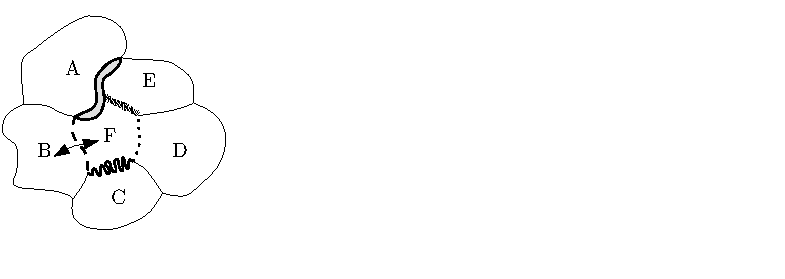
\includegraphics[width=0.33\linewidth]{figs/dpm1}}
% \quad
\subfloat[]{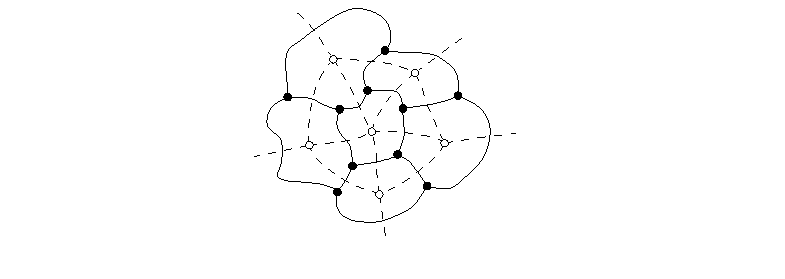
\includegraphics[width=0.33\linewidth]{figs/dpm2}}
% \quad
\subfloat[]{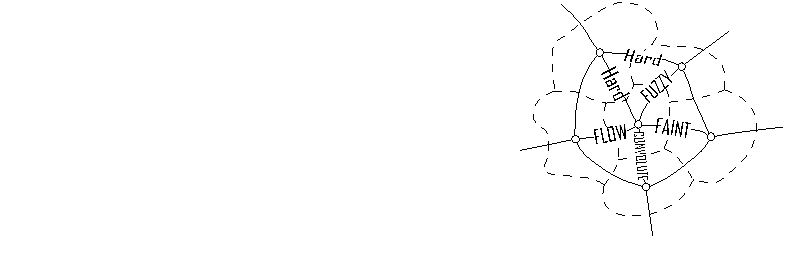
\includegraphics[width=0.33\linewidth]{figs/dpm3}}
\caption[Duality in a 2D map]{(a) Six map objects and their boundaries.
(b) The same map stored as a graph and its dual (dotted lines).
(c) The dual graph is used to describe the relationships between adjacent polygons.
From \citet[Ch.~6]{Ledoux06}, itself based on \citet{Gold91}.}
\label{fig:dual_polygonal_map}
\end{figure}

In three dimensions, duality characterises how volumes are related (\eg\ two neighbouring rooms in a building are adjacent).
It is most commonly used to model paths inside 3D buildings, which can be used for navigation computations.
\citet{Lee08} and \citet{Lee08a} extract from a 3D building a graph that can be used in case of emergency, and \citet{Boguslawski11a} and \citet{Boguslawski11} perform the same using the \emph{dual half-edge} data structure, which simultaneously represents the buildings (the rooms and their boundaries) and the navigation graph.
A typical example involves the Delaunay triangulation and the Voronoi diagram, which are dual to each other.
\citet{Dakowicz03} use them for terrain modelling, \citet{Lee02} for interactive analysis, and \citet{Ledoux08} for three-dimensional fields in the geosciences.

In four dimensions and higher, duality similarly characterises relationships between objects, albeit its exact meaning depends on the characteristics being modelled as dimensions.
For instance, in a 3D space+time setting, where a 4-cell represents a volume existing through time, the adjacency relationships between 4-cells represent volumes that were adjacent \emph{during one or more time intervals}.
These relationships can thus be used to answer connectivity questions in space-time without added semantics in the model.
For instance, it would make it possible to create a 3D indoor and outdoor way-finding application, where a user can select any given start and end points, and be given the best 3D route at any point in time, taking into account topological changes (\eg\ a connecting corridor being only open during office hours).

In a dimension-independent setting, generalised and combinatorial maps are notable because at the same time they encode a cell complex and its dual.
As shown in \reffig{fig:dual_gmap}, if an $n$-dimensional cell complex is stored as an $n$-dimensional generalised map, swapping $\alpha_n$ and $\alpha_{n-i}$ for every $i$ for every dart, the dual of the map is obtained\footnote{However, does not need to actually swap $\alpha_n$ and $\alpha_{n-i}$, but merely to \emph{consider} $\alpha_n$ as $\alpha_{n-i}$.}.
Note however that as shown in \reffig{subfig:dual_gmap2}, it is in practice necessary to compute a new point embedding that lies in the interior of every $n$-cell.
\begin{figure}[tb]
\centering
\subfloat[]{
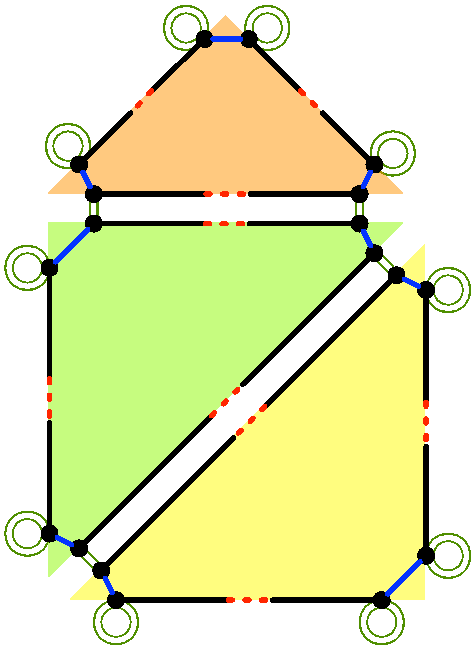
\includegraphics[width=0.21\linewidth]{figs/dual_gmap1}
\label{subfig:dual_gmap1}}
\quad
\subfloat[]{
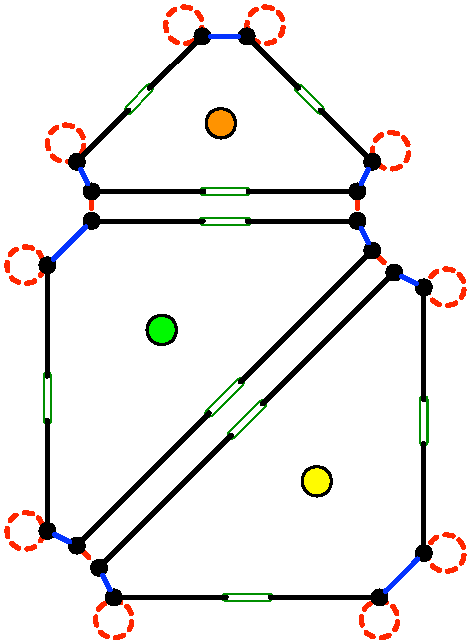
\includegraphics[width=0.21\linewidth]{figs/dual_gmap2}
\label{subfig:dual_gmap2}}
\quad
\subfloat[]{
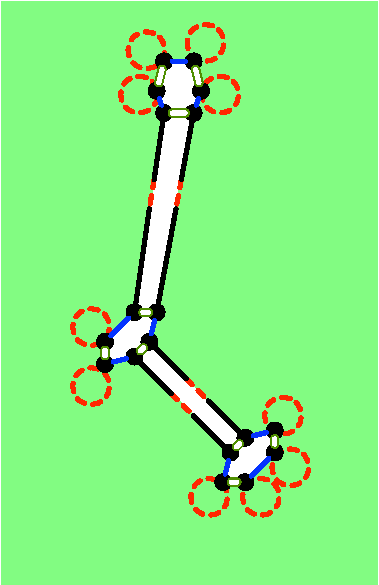
\includegraphics[width=0.21\linewidth]{figs/dual_gmap4}
\label{subfig:dual_gmap4}}
\quad
\subfloat[]{
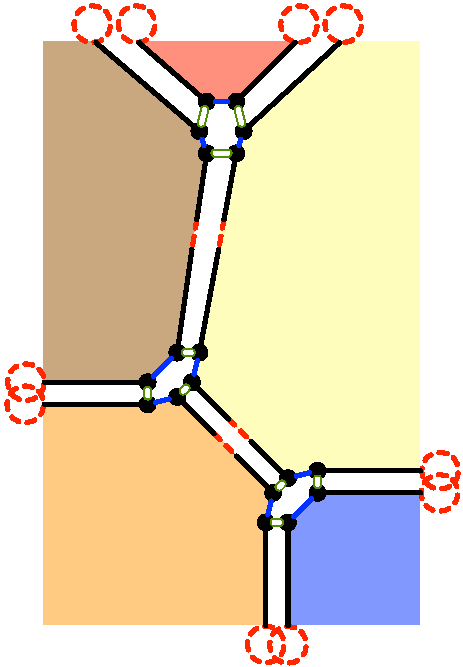
\includegraphics[width=0.21\linewidth]{figs/dual_gmap3}
\label{subfig:dual_gmap3}}
\caption[A 2D generalised map and its dual]{The dual of (a) a 2D generalised map can be obtained by (b) computing a point location for the dual 2-cells (\eg\ their centroid) and swapping $\alpha_0$ and $\alpha_2$, and (c) considering the 2-cells as 0-cells with their new point embeddings.
By extending every the exterior of (a) as an additional unbounded face, it is possible to arrive at the alternative dual map in (d).}
\label{fig:dual_gmap}
\end{figure}

\section{Comparing two objects with and without signatures}
\label{se:ndqueries}

In order to showcase the difference between topological and non-topological approaches in representing higher dimensional spatial information, this section compares how efficient the two approaches are in terms of size, and how efficiently three fundamental operations can be performed in either case.
The configurations for these tests are shown in \reffig{fig:tesseract-tests} and respectively involve verifying that two tesseracts are: equal (\ie\ that they represent the same 4-cell), adjacent (\ie\ that they share a common 3-cell face), and sharing a common 2-cell ridge.
As an example of the topological approach, objects will be represented as a combinatorial map with indices on the lexicographically smallest vertex of every cell.
Meanwhile, the non-topological approach will be exemplified with the Simple Features-like \citep{SimpleFeatures1} representation shown in \refse{ss:nd-topology} and \reffigp{fig:sfsnd}.
Indices make little sense in the latter, as there are no combinatorial primitives to navigate and every lower-dimensional cell is represented multiple times.

\begin{figure}[tb]
\centering
\subfloat[]{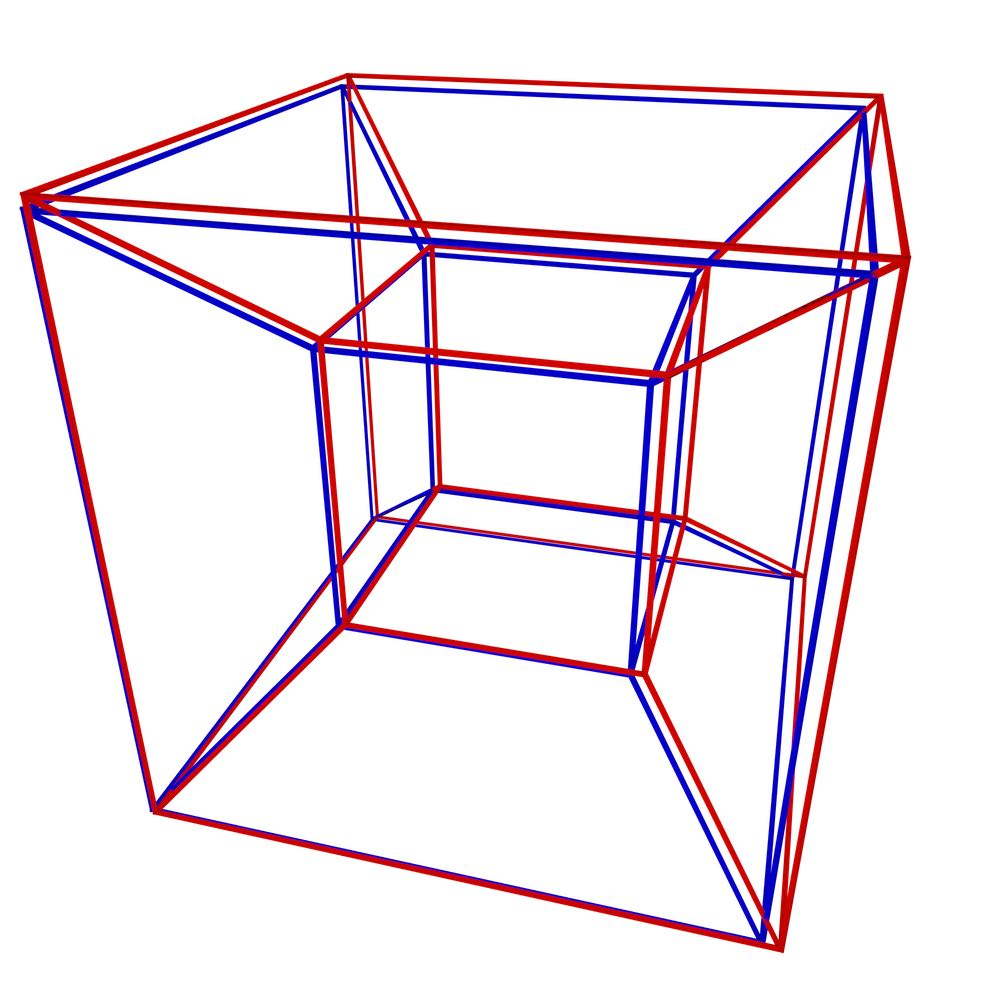
\includegraphics[width=0.33\linewidth]{figs/tesseract-tests-1}}
% \quad
\subfloat[]{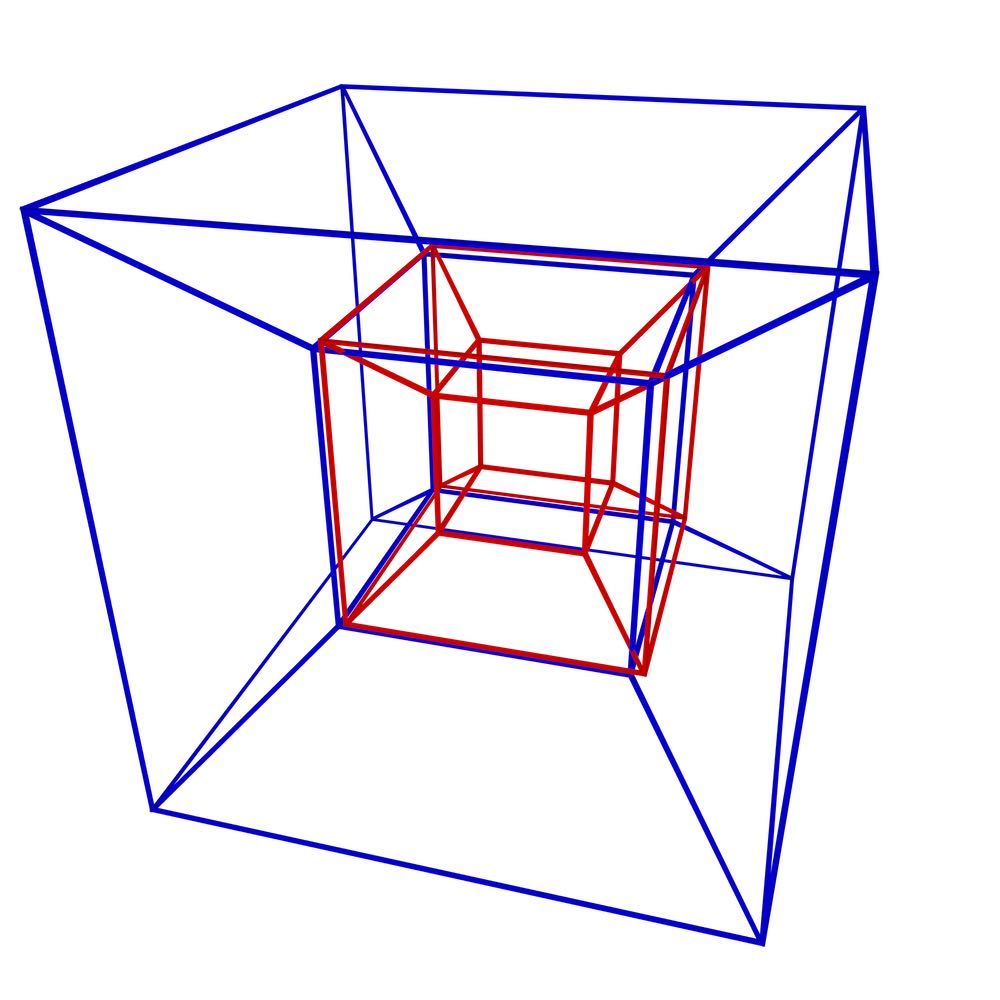
\includegraphics[width=0.33\linewidth]{figs/tesseract-tests-2}}
% \quad
\subfloat[]{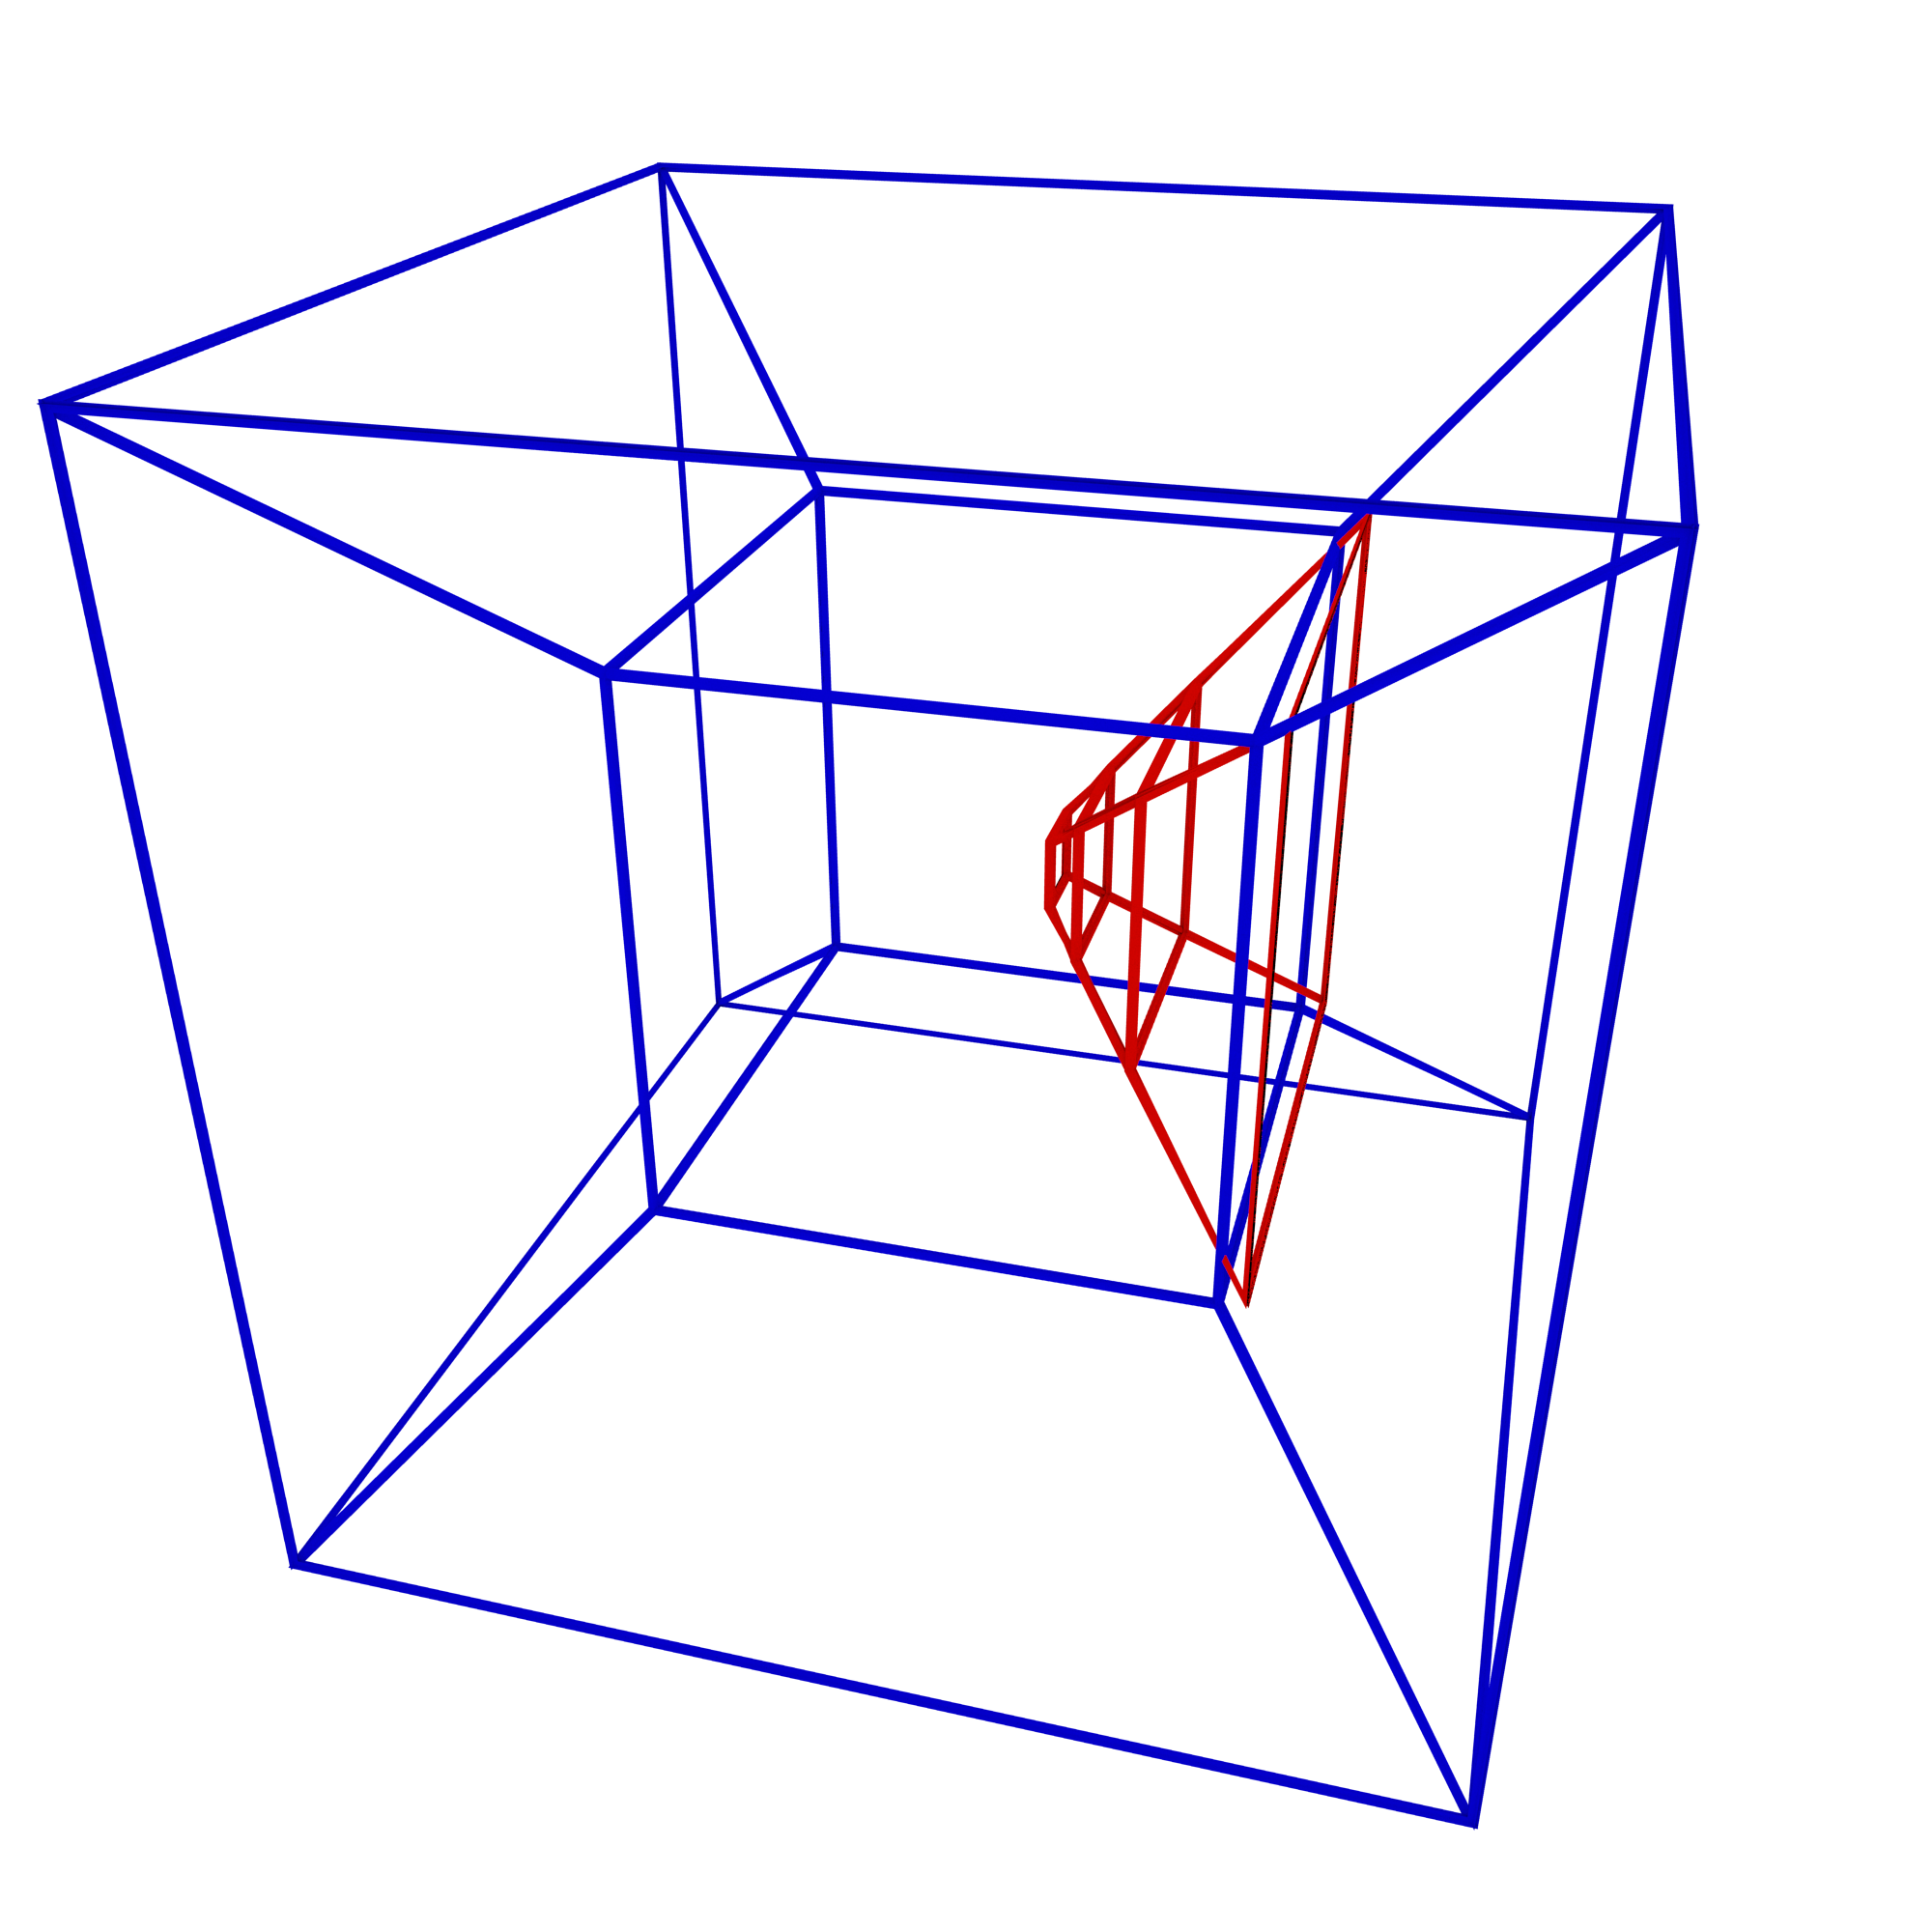
\includegraphics[width=0.33\linewidth]{figs/tesseract-tests-3}}
\caption[Three pairs of tesseracts]{A stereographic projection of three pairs of tesseracts representing: (a) equality (common 4-cell), (b) adjacency (a common 3-cell), and (c) common 2-cell. Only the edges of each tesseract are shown.}
\label{fig:tesseract-tests}
\end{figure}

The tests involving comparisons of combinatorial maps use the method of \citet{Gosselin11}, which can be used to compare two orbits of a map using \emph{signatures}.
This method will also be used extensively in \refch{ch:incremental-construction}.
Based on the ordering properties of a map, it is possible to traverse a given orbit from a given dart in a manner that is always consistent, yielding a canonical representation.
By following parallel traversals of this type, an algorithm can verify that two cells or maps are isomorphic in $O(n^2)$ time on the number of darts in a cell/map.

Intuitively, the quadratic complexity reflects the fact that two cells/maps are tested for isomorphism by starting one traversal always at the same dart in one of the cells/maps, possibly including a comparison of up to $n$ darts, while trying all $n$ possible starting darts in the other cell/map.
However, it is worth noting that most of the comparisons will stop as soon as one test fails, yielding a much better complexity in all but the most pathological cases.
Interestingly, \citet{Gosselin11} also provides a method to verify an isomorphism in $O(n)$ time on a specially generated external signature that uses $O(n^2)$ space, but this method is deemed too space-intensive for the purposes of this thesis.

All tests are described in detail below.

\subsection*{Size comparison}

Comparing the size of each structure is rather difficult as it can vary greatly depending on the specific implementation.
The specific implementations described below should nevertheless be roughly comparable, as they are tailored to the data but do not hard-code any specific object.

\begin{description}
\item[Combinatorial map] A combinatorial maps representation of a tesseract (\reffigp{fig:tesseract-darts}) is represented as 192 darts and 16 point embeddings.
Stored in a 3D combinatorial map\footnote{There is no need for a 4D combinatorial map, as there is only one 4D object.}, every dart contains links to 4 other darts ($\beta_1$ to $\beta_3$ plus $\beta_1^{-1}$) and to its point embedding.
As every point is embedded in 4D, every point embedding must store 4 coordinates.
Assuming that dart and point embedding links are stored as indices (\eg\ of an array) using 1 byte and point coordinates are stored using 4 bytes, a tesseract is stored in exactly 1 Kb of memory.

\item[Simple Features] A Simple Features representation of a tesseract (\reffigp{subfig:sfs4d}) contains 8 lists representing its bounding cubes, each of which contains 6 lists representing the bounding squares of a cube, each of which contains 5 lists representing a cycle of points on its boundary, each of which contains the 4 coordinates of a point.
Assuming that the first three levels of the lists (\ie\ 4D, 3D and 2D) are implemented as arrays that use one more item than their contents\footnote{In order to know the structure of the lists, it is necessary to terminate them with a special character (\eg\ the \texttt{'\textbackslash0'} null terminator used in C strings) or putting their size as their first element. Both of these options use one more item than their contents. Using a linked list would be much less efficient.} and the last level (\ie\ the point coordinates) as arrays of four elements and point coordinates are stored using 4 bytes, a tesseract is stored in 5.9 Kb of memory.
% ---\emph{5.9 times more than in a combinatorial map}.
\end{description}

\subsection*{Equality test}

\begin{description}
\item[Combinatorial map] In two equal tesseracts, the lexicographically smallest vertex is the same for both of them.
Using the index, it is possible to get a dart at the lexicographically smallest vertex in each.
As 4 cubes in each contain this vertex, and 3 faces of each of these cubes contain it, there are 12 darts that are embedded there.
Using the isomorphism test using signatures, this would mean 12 possible starting darts in one tesseract's traversal (the other is fixed), each of which can be performed in 2 orientations.
As these traversals can be of up to 192 darts, and each dart comparison involves 4 $\beta$-links and a point embedding with 4 coordinates, the process might include up to 36 864 comparisons.

\item[Simple Features] It is possible to test for equality by traversing one tesseract in order, point by point, while searching for an equivalent point in the other tesseract.
As the first two levels of their lists can be in any order (\ie\ 4D and 3D) and the third level list (\ie\ 2D) can have any starting point, there are 240 possible starting points from which a parallel traversal in the other tesseract can be started, which can be done in 2 possible orientations (forward and backward in every face cycle).
These traversals can include up to 240 points, each including up to 4 coordinate comparisons, yielding a total of up to 460 800 comparisons.
\end{description}

\subsection*{Adjacency test}

\begin{description}
\item[Combinatorial map] A tesseract has 8 cubical 3-cells, any of which can be equivalent to a 3-cell in the other tesseract.
A worst case test thus involves 32 cube-to-cube comparisons.
Comparing two cubes involves a similar process as the one described above for a tesseract.
Using indices, it is possible to arrive at the 3 darts at the lexicographically smallest vertex of each cube, from which comparisons can be started in 2 orientations, which involve traversals of up to 24 darts.
Each dart comparison involves 3 $\beta$-links ($\beta_3$ does not need to be tested) and a point embedding with 4 coordinates, yielding 1 008 comparisons per cube-to-cube test and 32 256 total.

\item[Simple Features] There are also 32 possible cube-to-cube comparisons to be made, each of which is also analogous to the tesseract comparison used above.
In a cube (\reffigp{subfig:sfs3d}), there are 30 possible starting points for a parallel traversal in 2 possible orientations, each involving up to 30 points with 4 coordinates.
Each cube-to-cube comparison thus involves 7 200 comparisons, for a total of 230 400.
\end{description}

\subsection*{Common 2-cell test}

\begin{description}
\item[Combinatorial map] Each tesseract has 24 square 2-cells, so there are 288 possible square-to-square comparisons.
There is only 1 dart at the lexicographically smallest vertex of each square, from which a comparison can be started in 2 orientations, involving up to 4 darts with 2 $\beta$-links and a point with 4 coordinates.
There are thus 48 comparisons per square-square combination and 13 824 total.

\item[Simple Features] There are also 288 possible square-to-square comparisons.
In a square (\reffigp{subfig:sfs2d}), there are 5 possible starting points for a traversal in 2 orientations, each involving 5 other points with 4 coordinates.
A square-to-square comparison thus involves 200 comparisons, for a total of 57 600.
\end{description}

\subsection*{Conclusions and insights into tests in higher dimensions}

\reftab{table:comparison-tests} summarises the results of the previous tests.
As the table shows, a topological approach using combinatorial maps is significantly more efficient than a non-topological Simple Features-like approach.
This is true both in terms of size and the number of comparisons involved in basic operations.
The difference ranges from a factor of 4.17 for detecting a common 2-cell ridge to a factor of 12.5 for detecting equality (\ie\ a common 4-cell).

\begin{table}[tbp]
\caption[Tesseract comparison test results]{The relative sizes and maximum number of comparisons in tests with two tesseracts (\reffig{fig:tesseract-tests}) using combinatorial maps (c-maps) and a Simple Features Specification (SFS) representation.}
\centering
\small
\begin{tabular}{cccc}
\toprule
Test & c-maps & SFS & factor \\
\midrule
size (Kb) & 1 Kb & 5.9 Kb & 5.9 \\
equality (comparisons) & 36 864 & 460 800 & 12.5 \\
adjacency (comparisons) & 32 256 & 230 400 & 7.14 \\
common 2-cell (comparisons) & 13 824 & 57 600 & 4.17 \\
\bottomrule
\end{tabular}
\label{table:comparison-tests}
\end{table}

This difference only becomes more pronounced with more complex objects and those of higher dimensions, as the advantage of having an index pointing to a well-defined starting point for a traversal is inversely proportional to the number of possible starting points.